\chapter{Parallel Random Access Machine $(PRAM)$}

Model, ktorý predstavujeme v tejto kapitole, je najviac podobný
reálnym paralelným architektúram. Ide o sústavu veľa (teoreticky
nekonečne) samostatných výpočtových jednotiek, ktoré nazývame
procesory. Každý procesor má svoju privátnu pamäť a sadu
inštrukcií podobných tým, ktoré poznáme z asembleru. Jednotlivé
procesory spolu komunikujú cez spoločnú zdielanú pamäť. Tento
model je akousi automatovou analogiou k modelu $PCGS$.
\\ Nebudeme sa zaoberať porovnávaním generatívnej sily $PRAMu$ s
modelmi Chomského\newline hierarchie, pretože už jeden samostatný
procesor $(RAM)$ má generatívnu silu Turingovho stroja. Zameriame
sa skôr na využitie sily tohto modelu na rýchle paralelné riešenie
problémov. V závere porovnáme model $PRAM$ s booleovskými obvodmi.

\section{Definície a označenia}

Skôr ako si zadefinujeme výpočtový model $PRAM$, s ktorým budeme
ďalej pracovať, povieme si niečo o jeho základnej základnej
výpočtovej jednotke, ktorou je $RAM$.

\subsection{$RAM$}

\begin{definicia}
$RAM$ (Random Access Machine) je výpočtový model pozostávajúci z
výpočtovej jednotky s pevne daným programom, jednej vstupnej a
jednej výstupnej pásky a neobmedzeného počtu registrov
$R_0,R_1,R_2,\dots$, pričom v jednom registri môže uchovávať
ľubovoľne veľké celé číslo (obr.\ref{pram_obr_modelram}). Program
výpočtovej jednotky je postupnosť jednoduchých\footnote{V sade
inštrukcií máme len jednoduché násobenie t.j. obsah registra krát
nejaká konštanta. Nemáme tu násobenie medzi registrami, lebo to by
dalo modelu $RAM$ príliš veľkú silu.} inštrukcií, ktoré sú uvedené
v tabuľke \ref{pram_tab_ram}. Výpočet začína prvou inštrukciou a
končí inštrukciou HALT.
\end{definicia}

\begin{figure}[!ht]
 \centering
 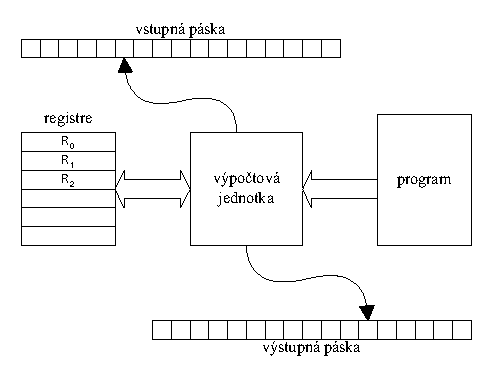
\includegraphics{img/pram/modelram.eps}
 \caption{Model $RAM$} \label{pram_obr_modelram}
\end{figure}

\begin{table}[!ht]\label{pram_tab_ram}
 \begin{center}
  \begin{tabular}{|c||c|}
   \hline
   inštrukcia & popis \\  \hline  \hline
   $READ$ & prečítaj nasledujúci symbol zo vstupu a zapíš ho do
   registra $R_0$ \\ \hline
   $WRITE$ & obsah registra $R_0$ zapíš na výstup \\ \hline
   $STORE\; R_i$ & obsah registra $R_0$ zapíš do registra $R_i$ \\
   \hline
   $COPY\; R_i$ & skopíruj obsah registra $R_i$ do registra $R_0$
   ($R_0\leftarrow [R_i]$) \\ \hline
   $CONST\; c$ & do registra $R_0$ zapíš hodnotu $c$ \\ \hline
   $ADD\; R_i$ & $R_0\leftarrow [R_0]+[R_i]$ \\ \hline
   $SUB\; R_i$ & $R_0\leftarrow [R_0]-[R_i]$ \\ \hline
   $MULT\; c$ & $R_0\leftarrow [R_0].c$ \\ \hline
   $DIV\; c$ & $R_0\leftarrow [R_0]/c$ \\ \hline
   $IFZERO\; i$ & ak register $R_0$ obsahuje 0, tak pokračuj
   inštrukciou $i$ \\ \hline
   $GOTO\; i$ & pokračuj inštrukciou $i$ \\ \hline
   $HALT accept$ & ukonči výpočet a akceptuj\\ \hline
   $HALT reject$ & ukonči výpočet a neakceptuj\\ \hline
  \end{tabular}
 \end{center}
\caption{Zoznam jednoduchých inštrukcií $RAMu$}
\end{table}

Model $RAM$ sa dá zadefinovať viacerými spôsobmi. Uvedenú
definíciu môžme, bez zmeny výpočtovej sily a zložitosti,
modifikovať tak, že vstup nebude zadaný na vstupnej páske, ale v
špeciálnych registroch, pričom v jednom z nich bude zadaná veľkosť
vstupu $n$ a v ďalšich $n$ registroch bude bit po bite zadaný
samotný vstup. \\ Ďalšou modifikáciou môže byť rovnakým spôsobom
upravený výstup, teda nie na výstupnej páske, ale opäť v (na to
určených) registroch.

\subsection{$PRAM$}

Prirodzeným rozšírením modelu $RAM$ v paralelných výpočtoch je
model $PRAM$, ktorý v sebe integruje viacero $RAMov$
komunikujúcich prostredníctvom zdieľanej pamäte.

\begin{figure}[!ht]
 \centering
 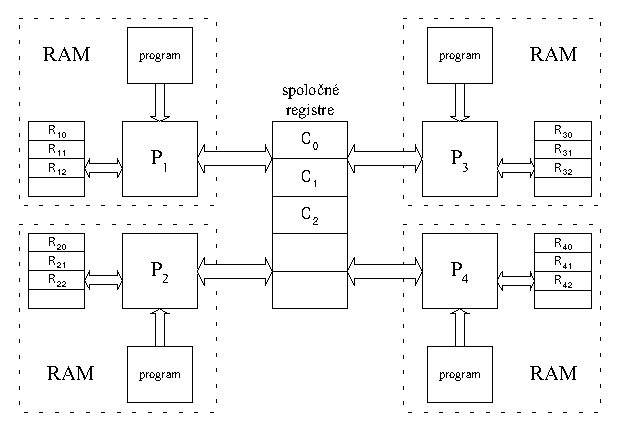
\includegraphics{img/pram/modepram.eps}
 \caption{Model $PRAM$} \label{pram_obr_modelpram}
\end{figure}

\begin{definicia}
$PRAM$ (Parallel Random Access Machine) je výpočtový model
pozostávajúci z neobmedzeného počtu $RAM$ procesorov označených
$P_0,P_1,P_2,\dots$ a neobmedzeného počtu spoločných (zdieľaných)
registrov $C_0,C_1,C_2,\dots$ Každý procesor $P_i$ má svoje
identifikačné číslo (index), má svoju vlastnú pamäť t.j.
ne\-ob\-me\-dze\-nú sadu registrov $R_{i,0},R_{i,1},R_{i,2},\dots$
a inštrukcie na priamy alebo nepriamy prí\-stup (read/write) do
spoločnej pamäte. Základná sada inštrukcii je zobrazená v tabuľke
\ref{pram_tab_pram}. Procesory sú zosynchronizované podľa globálnych
hodín, teda inštrukcie\linebreak v jednotlivých procesoroch sú
vykonávané v taktoch.
\\ Vstup $x\in\{ 0,1\}^n$ je zadaný nasledovne:
\begin{itemize}
  \item v registri $C_0$ je uložená dĺžka vstupu $n$
  \item v registri $C_i$ je uložený i-ty bit vstupu $x_i$
\end{itemize}
Výstup $y\in\{ 0,1\}^m$ je uložený v rovnakej forme.
\end{definicia}

\begin{table}[!ht]\label{pram_tab_pram}
 \begin{center}
  \begin{tabular}{|c||c|}
   \hline
   inštrukcia & popis \\  \hline  \hline
   $R_i\leftarrow [R_j]$ & skopíruj obsah registra $R_j$ do registra $R_i$
   \\ \hline
   $IDENT$ & do registra $R_0$ zapíš číslo procesora \\ \hline
   $CONST\; c$ & do registra $R_0$ zapíš hodnotu $c$ \\ \hline
   $ADD\; R_i$ & $R_0\leftarrow [R_0]+[R_i]$ \\ \hline
   $SUB\; R_i$ & $R_0\leftarrow [R_0]-[R_i]$ \\ \hline
   $MULT\; c$ & $R_0\leftarrow [R_0].c$ \\ \hline
   $DIV\; c$ & $R_0\leftarrow [R_0]/c$ \\ \hline
   $IFZERO\; i$ & ak register $R_0$ obsahuje 0, tak pokračuj
   inštrukciou $i$ \\ \hline
   $GOTO\; i$ & pokračuj inštrukciou $i$ \\ \hline
   $HALT$ & ukonči výpočet \\ \hline
  \end{tabular}
 \end{center}
\caption{Zoznam jednoduchých inštrukcií $PRAMu$}
\end{table}

\smallskip

Pri práve zadefinovanom modeli sa ukazujú dva závažné problémy:
\begin{enumerate}
  \item Nemôžeme predpokladať, že potenciálne nekonečne veľa
  procesorov sa bude podieľať na danom výpočte, a teda že budú
  všetky aktívne. Každý výpočet potrebuje isté množstvo
  procesorov, ktoré je závislé od vstupu resp. jeho dĺžky. Preto
  jeden z procesorov, označený ako $P_0$, má význačné postavenie,
  je to akýsi ``generál''. $P_0$ zapíše do špeciálneho registra $C_{-1}$
  maximálne číslo aktívneho procesora t.j. všetky procesory s
  menším indexom sú aktívne počas výpočtu. Teda najskôr je aktívny
  $P_0$ a ostatné čakajú, kým zapíše hodnotu maximálneho indexu
  procesora.\footnote{inou možnosťou riešenia tohoto problému by
  bolo zavedenie inštrukcie FORK, ktorou ľuboľný aktívny procesor môže
  aktivovať ďalšie, pričom na začiatku bude aktívny len procesor
  $P_0$}
  Výpočet skončí, keď skončí procesor $P_0$ t.j. vykoná HALT.
  \item Musíme vyriešiť konflikty pri viacnásobnom prístupe do
  spoločnej pamäte. Každá inštrukcia je vykonávaná v troch fázach.
  V prvej fáze je povolený prístup (ak treba) do spoločnej pamäte
  pre čítanie, potom sa vykoná príslušný výpočet pre danú
  inštrukciu, a nakoniec je povolený prístup (ak treba) do
  spoločnej pamäte pre zápis. Týmto sme oddelili prístup pre
  čítanie od prístupu pre zápis. Treba ešte vyriešiť situáciu, keď
  viac procesorov naraz pristupuje do spoločnej pamäte. Poznáme
  tri základné typy modelu $PRAM$:
  \begin{itemize}
    \item $CRCW-PRAM$ (Concurrent Read Concurrent Write) \\ Dovolíme
    procesorom súčasné čítanie aj súčasný zápis do spoločnej
    pamäte (registra). Tento typ má tri verzie:
    \begin{itemize}
      \item $PRIORITY:$ Ak chce do jedného registra zapisovať
      viacero procesorov, zápis vykoná len procesor s najmenším
      číslom z procesorov, ktoré žiadali o zápis.
      \item $COMMON:$ Ak chce do jedného registra zapisovať viacero
      procesorov, zápis sa uskutoční len vtedy, ak všetky
      procesory chcú zapísať rovnakú hodnotu.\newline V opačnom prípade sa
      výpočet zasekne.
      \item $ARBITRARY:$ Ľubovoľný\footnote{je to jediný
      nedeterministický prístup v modeli $PRAM$ t.j. môže sa stať,
      že pri opakovanom výpočte na rovnakom vstupe dostaneme
      rozdielne výstupy} z procesorov žiadajúcich o zápis zapíše
      svoju hodnotu do registra
    \end{itemize}
    \item $CREW-PRAM$ (Concurrent Read Exlusive Write) \\ Dovolíme\footnote{to
    znamená, že program (postupnosť inštrukcií) pre jednotlivé
    procesory musí spĺňať túto podmienku}
    procesorom súčasné čítanie spoločného registra, ale zapisovať do
    spoločného registra môže vždy len jeden procesor.
    \item $EREW-PRAM$ (Exlusive Read Exlusive Write) \\ Čítať a zapisovať do
    spoločného registra môže vždy len jeden procesor.
  \end{itemize}
\end{enumerate}

\section{Miery zložitosti}

Pri modeli $RAM$ uvažujeme tieto jenotkové miery zložitosti:
\begin{itemize}
  \item $TIME$ $T(n)$ = počet vykonaných inštrukcií
  \item $SPACE$ $S(n)$= počet použitých registrov
\end{itemize}
Z definície týchto mier je zrejmé, že neuvažujú veľkosť dát
(čísel), s ktorými inštrukcie pracujú, teda pracovať s veľkými
číslami je rovnako ``drahé'' ako pracovať s malými číslami. Z toho
plynie, že použitie jednotkovej miery nie je vhodné napr. pri
porovnávaní $RAM$ s Turingovým strojom. V takýchto prípadoch
uvažujeme tzv. logaritmickú mieru, ktorá zohľadňuje veľkosti čísel
pri jednotlivých operáciach. Logaritmická miera sa však používa
len zriedka, lebo v praxi máme aj tak obmedzenú veľkosť aj počet
registrov.

\pagebreak

Pri modeli $PRAM$ uvažujeme tieto jenotkové miery zložitosti:
\begin{itemize}
  \item $TIME$ $T(n)$ = počet krokov (taktov) procesora $P_0$ pri
  výpočte na vstupe dĺžky $n$
  \item $PROCESSORS$ $P(n)$ = maximálny počet aktívnych procesorov
  počas výpočtu na vstupe dĺžky $n$
\end{itemize}

Model $PRAM$ nemôže generovať príliš veľké (superpolynomiálne)
čísla. To znamená, že po $T(n)\leq \log n$ taktoch nebude ani v
jednom registri zapísané číslo s viac ako $O(T(n))$
bitmi.\linebreak Z toho plynie, že pri výpočte s časovou
zložitosťou $T(n)$ na $P(n)$ procesoroch $PRAM$ nespotrebuje na
uloženie dát viac ako $O(P(n).T^2(n))$ bitov. Máme teda adekvátnu
mieru pre pamäťové nároky $(SPACE)$.

\section{Výpočtová sila modelu $PRAM$}

Najskôr si ukážeme niekoľko príkladov výpočtov na modeli $PRAM$.

\begin{priklad}
Chceme vypočítať maximum z postupnosti $n$ zadaných čísel
$x_1,\dots ,x_n$ na\linebreak modeli $COMMON$ $CRCW-PRAM$.
\\ Vstup bude zadaný nasledovne: $C_0\leftarrow n$, $C_1\leftarrow
x_1,\dots ,C_n\leftarrow x_n$.
\\ Chceme\footnote{$[C]$ označuje obsah registra $C$, $C\leftarrow
a$ označuje zápis čísla $a$ do regitra $C$} výstup: $[C_0]=\max \{
x_1,\dots ,x_n\}$.
\\ Na výpočet použijeme $n^2$ procesorov ozn. $P_{i,j}$, kde
$i,j\in\{ 1,\dots ,n\}$ plus procesor $P_0$:
\begin{enumerate}
  \item Každý procesor $P_{i,1}$ vykoná: $C_{n+i}\leftarrow 0$
  \item Každý procesor $P_{i,j}$ vykoná\footnote{procesor nemá k dispozícii
  takú silnú inštrukciu, ale iste si vieme predstaviť jej simuláciu pomocou konečného
  počtu $PRAM$-inštrukcií}: $if\; [C_i]<[C_j]\; then\; C_{n+i}\leftarrow 1$
  \\ Uvedomme si, že tu nenastane žiadny konflikt pri súčasnom
  zápise viacerých procesorov do toho istého registra, pretože
  všetky procesory, ktoré budú chcieť zapísovať do registra
  $C_{n+i}$, budú chcieť zapísať 1.
  \item Každý procesor $P_{i,1}$ vykoná: $if\; [C_{n+i}]=0\;
  then\; C_0\leftarrow [C_i]$
  \\ Po kroku 2 je medzi registrami $C_{n+1},\dots ,C_{2n}$ jediný
  s nulovou hodnotou a platí
  \\ $[C_{n+i}]=0$ práve vtedy, keď $x_i=\max\{x_1,\dots ,x_n\}$
\end{enumerate}
Ako vidieť, vďaka použitiu polynomiálneho počtu procesorov, sa nám
podarilo nájsť maximum\linebreak z číselnej postupnosti v
konštantnom čase. Pri sekvenčných modeloch na to potrebujeme
lineárny čas.
\end{priklad}

\begin{priklad}
\label{pram_prikl_2}

Opäť chceme vypočítať maximum ako v predchádzajúcom príklade, ale
tentoraz na modeli $EREW-PRAM$.
\\ Vstup je zadaný tak isto ako v predchádzajúcom príklade.
Budeme\footnote{rovnakú myšlienku možno použiť pri úlohe sčítať
$n$ čísel} porovnávať dvojice registrov, pričom výsledky zapíšeme
do nových registrov, ktoré budeme opäť po dvojiciach porovnávať
atď. takže dostaneme binárny porovnávací strom
(obr.\ref{pram_obr_maxstrom}). Keďže používame stále nové a nové registre a
každý register má na starosti jeden procesor, tak procesory naraz
nečítajú ani nezapisujú do toho istého registra.

\begin{figure}[!ht]
 \centering
 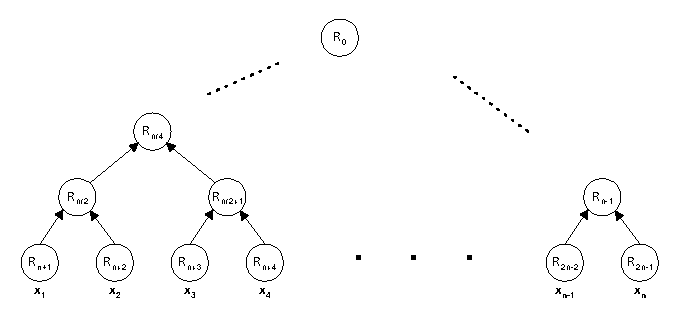
\includegraphics{img/pram/maxstrom.eps}
 \caption{Výpočet maxima na $EREW-PRAM$} \label{pram_obr_maxstrom}
\end{figure}

Procesorovú zložitosť sme zmenšili $P(n)=n$, ale časová zložitosť
vzrástla $T(n)=\log n$.
\end{priklad}

\begin{priklad}
Ukážeme si, ako efektívne vieme triediť postupnosť čísel
$x_1,\dots ,x_n$ na modeli $CREW-PRAM$.
\\ Vo vstupných registroch $C_1,\dots ,C_n$ sú hodnoty $x_1,\dots
,x_n$. Chceme, aby po skončení výpočtu boli v registroch
$C_1,\dots ,C_n$ čísla zo vstupu v utriedenom poradí.
\\ Na výpočet použijeme $n^2$ procesorov ozn. $P_{i,j}$.
\begin{enumerate}
  \item Každý procesor $P_{i,j}$ vykoná: $if\; [C_i]<[C_j]\; then\;
  C_{i,j}\leftarrow 1\; else\; C_{i,j}\leftarrow 0$
  \item Každých $n$ procesorov $P_{i,1},\dots ,P_{i,n}$ sa bude
  podieľať na výpočte\footnote{sčítať $n$ čísel je podobný problém
  ako nájsť maximum z $n$ čísel (príklad \ref{pram_prikl_2})}:
  $C_{n+i}\leftarrow 1+$ $\sum\limits_{j=1}^{n} [C_{i,j}]$
  \item Každý procesor $P_{i,1}$ vykoná: $C_{C_{n+i}}\leftarrow [C_i]$
\end{enumerate}
Časová zložitosť $TIME$ je $T(n)=O(\log n)$, lebo prvý a tretí
krok výpočtu trvá konštantný čas a na druhý potrebujeme
logaritmický čas, počet procesorov je $P(n)=n^2$.
\\ Teraz ľahko vidíme, že problém triedenia je v $\mathcal{NC}$,
teda ho vieme efektívne paralelne riešiť.
\end{priklad}

\medskip
Jednotlivé modely $PRAM$ sú medzi sebou relatívne ekvivalentné,
takže je v zásade jedno, ktorý používame. Tento poznatok využijeme
pri porovnaní $PRAM$ s booleovskými obvodmi. Teraz si ukážeme
porovnanie medzi modelmi $EREW$ a $CRCW$.

\begin{veta}
$\mathcal{L}(EREW-PRAM)=\mathcal{L}(CRCW-PRAM)$
\end{veta}

\begin{dokaz}
Inklúziu $\subseteq$ netreba dokazovať, pretože z definícií
jednotlivých modelov vyplýva, že $EREW$ je špeciálnym prípadom
$CRCW$. Dokážeme opačnú inklúziu.
\\ Chceme simulovať $CRCW$ na $EREW$. Treba vyriešiť
situáciu, keď viacero procesorov chce naraz zapisovať do toho
istého registra t.j. treba z nich vybrať jeden, ktorý svoju
hodnotu do registra naozaj zapíše. Budeme z nich vyberať procesor
s najmenším číslom (takto vyriešime naraz všetky tri verzie modelu
$CRCW$).
\\ Pod každým registrom $C_i$ budeme mať binárny strom
pozostávajúci z nových registrov obsahujúcich čísla procesorov. V
listoch sú čísla všetkých aktívnych procesorov. Na začiatku každý
procesor pozná svoju pozíciu v tomto strome. Nie každý aktívny
procesor chce v danom okamihu zapisovať do $C_i$. Budeme postupne
po dvojiciach porovnávať obsahy registrov v tomto strome.
\\ Ak je procesor ľavý (t.j. s menším číslom) a chce zapisovať do $C_i$,
tak postúpi o úroveň vyššie (t.j. zapíše do príslušného registra
svoje číslo).
\\ Ak je procesor pravý, tak ``skúsi'', či jeho ľavý sused
postúpil.\footnote{To môžeme zabezpečiť tak, že každý postup o
úroveň vyššie bude prebiehať v troch krokoch. V prvom ľaví z
dvojice buď nechcú zapisovať a nepostupujú alebo postúpia, ak chcú
zapisovať, zatiaľ čo praví čakajú t.j. vykonajú inštrukciu NOP. V
druhom kroku praví, ak chcú zapisovať do $C_i$, tak čítajú obsah
registra zodpovedajúcemu vyššej úrovni. V treťom kroku praví, ak
zistili, že ľaví nezapísali svoje číslo do registra vyššej úrovne,
tak tam zapíšu svoje číslo.} Ak áno, tak v ďalšom už nechce
zapisovať do $C_i$, ak nie, tak postúpi o úroveň vyššie. Toto sa
vykonáva až ku koreňu stromu, teda ku koreňu sa dostane len jeden
procesor (s najmenším číslom z aktívnych procesorov, ktoré chceli
zapisovať do $C_i$) a ten zapíše svoju hodnotu do registra $C_i$.

Čítanie bude fungovať podobne, iba s tým rozdielom, že výpočet na
strome pod každým registrom sa bude vykonávať opačným smerom, aby
každý z procesorov, ktorý mal záujem čítať, sa dostal k $C_i$.

Keďže binárne stromy pod registrami majú výšku $\log P(n)$, tak
čítanie registra a zápis do registra sa z jedného kroku v modeli
$CRCW$ predĺži na $O(\log P(n))$ krokov v modeli $EREW$, a teda
čas $EREW$ modelu sa oproti $CRCW$ zhorší $O(\log P(n))$ násobne.
To je ale v celku dobrá simulácia.
\end{dokaz}

\section{Porovnanie modelov $BO$ a $PRAM$}

\begin{veta}
Nech $\{ C_n\}$ je $BC$-uniformná postupnosť booleovských obvodov
počítajúca funkciu $f_n:\{ 0,1\}^n\rightarrow\{ 0,1\}^m$ taká, že
$DEPTH(C_n)=(\log n)^{O(1)}$ a $SIZE(C_n)=n^{O(1)}$. Potom
existuje $CREW-PRAM$, ktorý počíta funkciu $f_n$ v čase
$T(n)=(\log n)^{O(1)}$ na $P(n)=n^{O(1)}$ procesoroch.
\end{veta}

\begin{dokaz}
Základná idea dôkazu spočíva v tom, že každé hradlo booleovského
obvodu $(BO)$ bude simulované jedným procesorom a každé spojenie
medzi hradlami (t.j. vstup resp. výstup)\linebreak v $BO$ bude
reprezentované jedným spoločným registrom. Potom každý procesor v
príslušnom takte, podľa hĺbky simulovaného hradla v $BO$, načíta
obsahy registrov prislúchajúce k vstupom simulovaného hradla,
vykoná daný výpočet podľa typu hradla, a následne zapíše výsledok
do registra prislúchajúceho k výstupu hradla (pozri obrázok
\ref{pram_obr_bopram3}, kde kružnice predstavujú procesory a obdĺžniky
registre). Tento register je zároveň vstupným registrom pre nejaký
iný procesor, ktorý simuluje ďalšie hradlo v $BO$.

\begin{figure}[!ht]
\centering
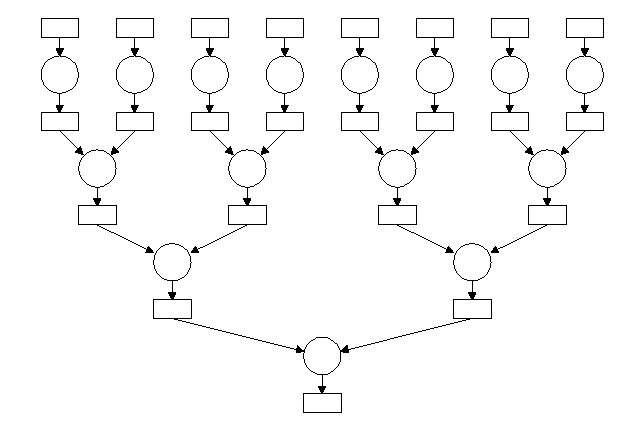
\includegraphics{img/pram/bopram3.eps}
\caption{Simulácia $BO$ na modeli $PRAM$} \label{pram_obr_bopram3}
\end{figure}

Každý procesor $P_i$, ktorý simuluje nejaké hradlo v $BO$, bude
mať v spoločnej pamäti vyhradené štyri registre $C_{i,IN1},
C_{i,IN2}, C_{i,OUT} ,C_{i,TYP}$, pričom v prvých dvoch budú
zapísané adresy dvoch vstupných registrov, do tretieho procesor
$P_i$ zapíše výstup a vo štvrtom bude zapísaný typ simulovaného
hradla. Procesor simulujúci vstupné hradlo samozrejme vystačí z
jedným registrom pre adresu vstupu.

Obsahy registrov $C_{i,IN1}, C_{i,IN2}, C_{i,TYP}$ závisia od
daného $BO$, a pred samotnou simuláciou ich podľa neho musíme
najskôr naplniť. Pripomeňme si, čo to znamená, že máme
daný\linebreak $BC$-uniformný booleovský obvod. Znamená to, že
poznáme $DTS\; A$ pracujúci s jednou\linebreak vstupnou, jednou
pracovnou a jednou výstupnou páskou, ktorý na vstupe $1^n$ zapíše
na výstupnú pásku kód $BO$ $C_n$, pričom pracovnú pásku má
obmedzenú na priestor $\log SIZE(C_n)$.

Chceme zostrojiť $PRAM$ simulujúci postupnosť $BO$ $\{ C_n\}$. To
znamená, že pre nejaký vstup dĺžky $n$ potrebujeme najskôr
odsimulovať výpočet $DTS\; A$, ktorý vygeneruje kód $BO$, potom ho
dekódovať (t.j. správne naplniť registre $C_{i,IN1}, C_{i,IN2},
C_{i,TYP}$), a nakoniec spustiť samotnú simuláciu výpočtu $BO$.

\pagebreak

\begin{itemize}
  \item Simulácia výpočtu $DTS\; A$:

  Čo vieme o $DTS\; A$? Ak uvažujeme, že $A$ pracuje na vstupe
  dĺžky $n$ v priestore\linebreak $S(n)=\log SIZE(C_n)$, tak počet všetkých
  možných konfigurácií $A$ je $k^{S(n)}.n.S(n)$ pre nejakú
  konštantu $k$, čo je rádovo $(SIZE(C_n))^{O(1)}$ čiže podľa
  predpokladu $n^{O(1)}$. Očíslujme si jednotlivé konfigurácie
  $1,2,\dots r$. Nech\footnote{takýto predpoklad môžeme urobiť,
  lebo pre daný vstup poznáme počiatočnú konfiguráciu a môžeme sa
  dohodnúť na jednej koncovej konfigurácií pre všetky výpočty, z
  ktorej sa už nedá dostať do inej konfigurácie} počiatočná
  konfigurácia má číslo $1$ a koncová má číslo $r$. Podľa
  predpokladu vety máme dostatok procesorov, aby sme každej
  konfigurácii priradili jeden procesor. Každému procesoru
  pridelíme dva registre zo spoločnej pamäte, jeden\footnote{POZOR:
  Nemýliť si s vyššie uvedeným rovnako nazvaným registrom,
  použitým pri samotnej simulácii $BO$} na výstup $(C_{j,OUT})$
  a druhý na číslo registra $(C_{j,REG})$.

  V prvom kroku každý procesor $P_j$ prislúchajúci j-tej
  konfigurácii odsimuluje jeden krok výpočtu $DTS\; A$ z tejto
  konfigurácie, pričom do prvého registra zapíše výstup
  zodpovedajúci tomuto kroku a do druhého zapíše číslo
  konfigurácie, do ktorej sa týmto krokom $A$
  dostal\footnote{tieto zápisy sú jednoznačné, keďže simulujeme
  deterministický stroj}. Keďže sme odsimulovali jeden krok $A$
  z každej konfigurácie, vyčerpali sme tým všetky možnosti
  $\delta$-funkcie, takže $\delta$-funkciu už simulovať
  nebudeme. V ďalšom chceme\linebreak jednotlivé kroky výpočtu $A$ vhodne
  ``pospájať'', aby spolu tvorili celý výpočet $A$, čím by sme
  dostali výsledný kód $\langle C_n\rangle$.

  V každom ďalšom kroku procesor $P_j$ vykoná:
  \begin{enumerate}
    \item  $C_{j,OUT}\leftarrow [C_{j,OUT}]\centerdot
    [C_{C_{j,REG},OUT}]$       , kde $\centerdot$ je
    zreťazenie\footnote{obsahmi registrov sú čísla v binárnom
    zápise, takže zreťazenie znamená nasledujúcu aritmetickú
    operáciu nad registrami: $C_{j,OUT}\leftarrow C_{j,OUT} +
    2^{|C_{C_{j,REG},OUT}|}.C_{C_{j,REG},OUT}$} obsahov registrov
    \item $C_{j,REG}\leftarrow [C_{C_{j,REG},REG}]$
  \end{enumerate}
  Každý procesor $P$ načíta registre procesora
  prislúchajúceho ku konfigurácii, ktorej číslo má procesor $P$ vo
  svojom druhom registri. Prvé (výstupné) registre zreťazí a toto
  zreťazenie zapíše ako novú hodnotu výstupného registra. Do
  druhého registra zapíše číslo konfi\-gurácie, ktoré načítal
  (obr.\ref{pram_obr_bopram1}). Každý procesor $P_j$ teraz reprezentuje dva
  kroky výpočtu $A$ začínajúci konfiguráciou číslo $j$. Po ďalšom
  kroku $PRAMu$ bude každý procesor $P_j$ reprezentovať štyri kroky
  výpočtu $A$ s výnimkou tých, ktoré už vo svojom druhom registri
  majú číslo koncovej konfigurácie, z ktorej sa už nedá dostať.
  Toto sa opakuje až kým procesor $P_1$ nemá vo svojom druhom
  registri hodnotu $r$. Vtedy sa simulácia generovania
  kódu\linebreak
  zastaví\footnote{realizáciu si môžeme predstaviť nasledovne:
  $P_1$ zapíše do nejakého špeciálneho booleovského registra, ktorý
  bol inicializovaný na TRUE, hodnnotu FALSE a program pre procesory
  upravíme tak, že dané inštrukcie budú vykonávať len vtedy, keď v
  tomto registri je hodnota TRUE} a $P_1$ bude mať vo svojom prvom
  registri celý výstup $A$, teda kód $BO$ $C_n$.
  Na obrázku \ref{pram_obr_bopram2} sú vyznačené procesory prislúchajúce ku
  konfiguráciám, v ktorých sa nachádza $DTS$ pri generovaní daného
  kódu. Hrubo vyznačené procesory sú pre nás významné z pohľadu
  generovania kódu. Tenko vyznačené procesory nám už nepomôžu k
  vygenerovaniu kódu, napriek tomu stále vykonávajú svoj program,
  pretože dopredu nevieme povedať, ktoré procesory budú významné a
  ktoré nie. Podobne nevieme dopredu určiť, ktoré procesory
  (konfigurácie) sa budú podielať na výpočte, a preto aj procesory,
  ktoré sa v konečnom dôsledku na výpočte podielať nebudú (na
  obrázku znázornené malými kružnicami v prvom riadku), vykonávajú
  svoj program.

\begin{figure}[!ht]
 \centering
 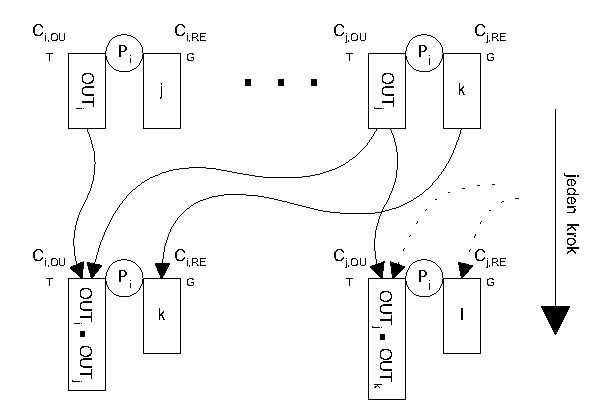
\includegraphics{img/pram/bopram1.eps}
 \caption{Jeden krok simulácie $DTS$} \label{pram_obr_bopram1}
\end{figure}

\begin{figure}[!ht]
 \centering
 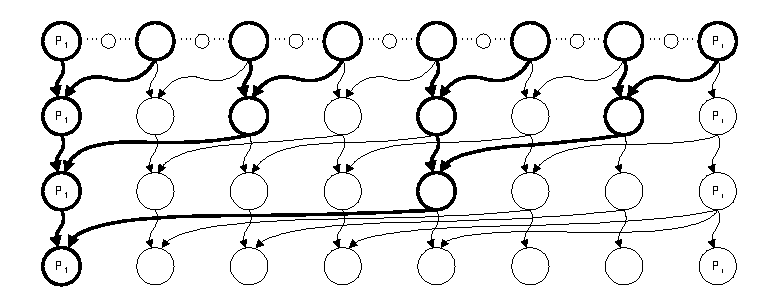
\includegraphics{img/pram/bopram2.eps}
 \caption{Generovanie kódu $BO$ na modeli $PRAM$} \label{pram_obr_bopram2}
\end{figure}

  Keďže po každom kroku $PRAMu$ sa dĺžka odsimulovaného výpočtu $A$
  zdvojnásobí, tak na odsimulovanie celého výpočtu vystačíme s
  časom logaritmus z počtu konfigurácií, čo je $O(\log
  SIZE(C_n))$.

  \item Dekódovanie:

  Predpokladajme, že už máme v nejakom registri kód $\langle C_n\rangle$. Ten
  je v tvare:

   \centerline{
  ($\langle$ číslo hradla,typ hradla,číslo ľavého vstupu, číslo
  pravého vstupu $\rangle$)$^*$}
  Zrejme dĺžka kódu je $|\langle C_n\rangle |=O(SIZE(C_n).
  \log SIZE(C_n))$. Opäť máme dostatok procesorov, aby sme nimi
  ``pokryli'' každý symbol výstupu. Každý procesor $P_j$ načíta
  register s kódom $\langle C_n\rangle$ a akoby nastaví svoju čítaciu
  hlavu na j-ty symbol kódu $\langle C_n\rangle$. Procesory samozrejme žiadne
  čítacie hlavy nemajú, ale ľahko si vieme predstaviť, že $PRAM$ by
  vedel na jeden krok ``rozložiť'' obsah registra na veľa registrov
  obsahujúcich po jednom symbole, a potom by už procesory pracovali
  nad registrami ako je to v modeli $PRAM$ zvykom a nie s čítacou
  hlavou ako prezentujeme tu.

  Po prvom kroku prestanú pracovať všetky procesory, ktoré
  neprečítali na vstupe symbol\footnote{všetky symboly sú zakódované
  binárne, takže procesory prestanú pracovať po tom ako rozpoznajú
  symbol ``(''} ``(''. Tie, ktoré ``('' prečítali
  (t.j. boli nastavené na začiatok podslova v kóde $\langle C_n\rangle$
  reprezentujúce kód nejakého hradla), v každom ďalšom kroku
  prečítajú jeden symbol, až kým neprečítajú ``)'' (t.j. koniec
  kódu hradla). Každý takýto procesor ``zistí'' informácie o
  jednom hradle $BO$, teda číslo hradla, typ hradla a čísla
  vstupov, a zapíše ich do príslušných registrov $C_{i,IN1},
  C_{i,IN2}, C_{i,TYP}$.

  Keďže čísla hradiel sú v kóde zapísané v binárnom tvare, tak
  dĺžka kódu jedného\linebreak hradla je $O(\log SIZE(C_n))$. Každý procesor
  potrebuje prečítať kód jedného hradla a\linebreak zapísať získané
  informácie do registrov. Preto čas, ktorý na dekódovanie
  potrebujeme, je $O(\log SIZE(C_n))$.

  \item Simulácia výpočtu $BO$:

  Teraz už máme všetko pripravené na simuláciu výpočtu $BO$, teda
  v registroch  $C_{i,IN1}$, $C_{i,IN2}$, $C_{i,TYP}$ sú zapísané
  správne hodnoty prislúchajúce simulovanému $BO$. Predpo\-kladajme,
  že všetky registre $C_{i,OUT}$ sú inicializované na nejakú
  NILovú hodnotu\footnote{vzhľadom na to, že vo výstupných
  registroch budú len hodnoty 0 alebo 1, hodnotu NIL môže
  reprezentovať akákoľvek iná hodnota}. Procesor $P_i$ bude
  vykonávať program:
  \begin{enumerate}
    \item načítaj obsahy registrov $C_{i,IN1}, C_{i,IN2}, C_{i,TYP}$
    \item čakaj kým platí: $[C_{C_{i,IN1}}] = NIL$ a $[C_{C_{i,IN2}}] = NIL$
    \item vykonaj operáciu podľa typu hradla $[C_{i,TYP}]$ so
    vstupmi $[C_{C_{i,IN1}}], [C_{C_{i,IN2}}]$
    \item zapíš výsledok operácie do registra $C_{i,OUT}$
  \end{enumerate}
  Na vykonanie tohto programu potrebuje každý procesor čas najviac
  $(\log n)^{O(1)}$, pretože na druhom riadku bude procesor čakať
  toľko krokov koľko je hĺbka hradla v $BO$ a z predpokladu vieme, že
  $DEPTH(C_n)=(\log n)^{O(1)}$, ostatné riadky programu sa
  vykonajú v konštantnom čase.
\end{itemize}

Z dôkazu ľahko vidieť, že sme splnili požiadavky kladené na časovú
a procesorovú zložitosť, ako aj na model $CREW-PRAM$.
\end{dokaz}

\begin{veta}
Nech $M$ je $CREW-PRAM$, ktorý v čase $T(n)={(\log n)}^{O(1)}$ a s
počtom procesorov $P(n)=n^{O(1)}$ počíta funkciu $f$. Potom
existuje konštanta $k$ a $BC$-uniformná postupnosť booleovských
obvodov $\{ C_n\}$ taká, že $C_n$ počíta na vstupe $x_1\dots x_n$
výstup $y_{11}y_{12}\dots y_{ij}\dots$ kde $y_{ij}$ je hodnota
j-teho bitu spoločného registra $C_i$ v čase $T(n)$ pre $1\leq
i\leq P(n).T(n)$ a $1\leq j\leq k.T(n)$, pričom $DEPTH(C_n)={(\log
n)}^{O(1)}$ a $SIZE(C_n)=n^{O(1)}$.
\end{veta}

\begin{dokaz}
Chceme zostrojiť $BO$ simulujúci $CREW-PRAM$. Vstupom pre $M$ je
prvých $n$ spoločných registrov $C_1,\dots ,C_n$. Vstupom
$x_1\dots x_n$ pre $BO$ $C_n$ sú obsahy týchto registrov\linebreak
v čase $T_0$.

Výpočet $M$ závisí od postupnosti inštrukcií jenotlivých
procesorov. Pre každú inštrukciu zostrojíme elementárny obvod
simulujúci túto inštrukciu. Vstupom preň bude obsah
registra\linebreak (registrov), s ktorým príslušná inštrukcia
pracuje a výstupom bude nový obsah výstupného registra. Uvedomme
si, že za nášho predpokladu existencie konštanty $k$ takej, že
$1\leq j\leq k.T(n)$ (t.j. vieme ohraničiť maximálnu veľkosť
registra počas celého výpočtu), každú inštrukciu vieme simulovať
elementárnym obvodom obsahujúcim konečný počet hradiel.

\begin{figure}[!ht]
 \centering
 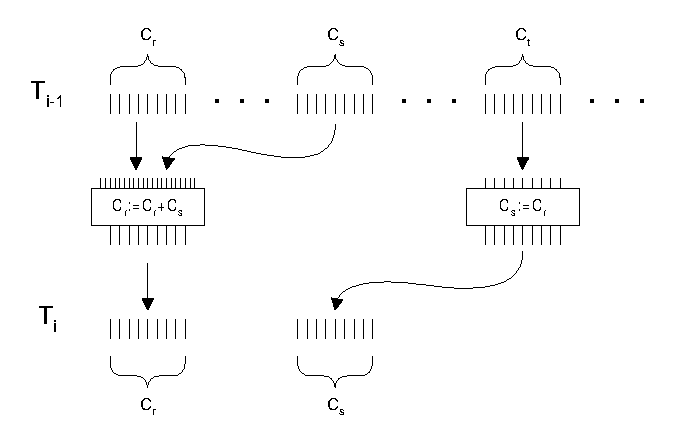
\includegraphics{img/pram/prambo.eps}
 \caption{Simulácia výpočtu $PRAM$ na $BO$} \label{pram_obr_prambo}
\end{figure}

$C_n$ bude mať $T(n)$ úrovní, pričom v i-tej úrovni budeme mať
obsahy všetkých registrov (bit po bite) v čase $T_i$. Dosiahneme
to tak, že medzi (i-1). úroveň a i-tu úroveň umiestnime (a vhodne
pospájame) elementárne obvody prislúchajúce k i-tym inštrukciám
všetkých aktívnych procesorov (obr.\ref{pram_obr_prambo}). Takže na
poslednej úrovni budú obsahy registrov v čase $T(n)$, čo zodpovedá
výstupu $M$.

Vďaka predpokladom o počte $(1\leq i\leq P(n).T(n))$, veľkosti
$(1\leq j\leq k.T(n))$ registrov a z toho vyplývajúcej konečnej
veľkosti elementárnych obvodov dostávame zložitosti pre $C_n$:
$DEPTH(C_n)={(\log n)}^{O(1)}$ a $SIZE(C_n)=n^{O(1)}$.

Teda dokázali sme ekvivalentnosť mier zložitosti medzi týmito
dvoma modelmi t.j. čas na modeli $PRAM$ zodpovedá hĺbke na $BO$ a
počet procesorov na $PRAM$ zodpovedá veľkosti $BO$.
\end{dokaz}

\begin{dosledok}
Model $PRAM$ je v druhej počítačovej triede.
\end{dosledok}

\begin{dosledok}
Triedu $\mathcal{NC}$ môžeme pomocou modelu $PRAM$ zadefinovať
nasledovne: \\ \centerline{$\mathcal{NC}=TIMEPROCESSORS((\log
n)^{O(1)},n^{O(1)})$}
\end{dosledok}
